\section{Detector Design and Selection}
\label{sec:3.1}
Our initial choice for a detector was to use a water level sensor which would use an raspberry pi to relay water depth over time. The water level is detected by measuring the change in voltage on the sensor traces caused by the conductive properties of water. When water bridges the gap between the sensor traces and the grounded traces, it pulls the sensor trace voltage low, indicating the presence of water. By using multiple traces at different heights, the sensor can estimate the water level \cite{noauthor_-depth_2019}\cite{noauthor_water_nodate}. The problem arose because the time interval between water level measurements was too long, allowing water to linger on the detector. This caused false positives when a wave passed over the sensor, as the residual water would maintain a low voltage reading even after the wave had receded. Hysteresis further exacerbated this issue, as the sensor's response lagged behind the actual water level changes, making it difficult to accurately detect the true water level during dynamic conditions like wave motion.

Another option was an ultrasonic sensor which would detect a difference in water level through ultrasonic waves reflecting off the waters surface \cite{noauthor_what_nodate}. Again, the issue was that the time interval between water level measurements was too long. We required a sensor that would report at a minimum of 20 times per second (see Appendix \ref{app:B}) to be able to produce reliable data where the time at which the wavefront was detected is accurate and changes in water level across the wave can be detected. 

We decided on using computer vision through a webcam recording at \ac{FPS} to then extract frames from the video feed. These frames would train a \ac{ML} model to detect wave movement through the motion of a bob placed on the surface of the water. This proved a much more reliable and consistent way of determining the motion of the wave and more importantly the time at which the wave crossed the detector. Its heightened response time and polling rate are both due to the webcam recording at 30 FPS, therefore the polling rate being $30$ times per second and its response time being $1/30 \space s$.

\section{Equipment Setup}

To simulate the propagation of GWs through space we use a simple setup of a container of water with measurements $W = 71.6 \space cm \pm0.1\space cm$ and $L = 43.3 \space cm \space \pm \space 0.1 \space cm$, as shown in Figure \ref{fig:setup}. To be able to measure the water level changes a small foam bob was placed into a glass tube suspended just above the water line, allowing the bob to move with the wave but keeping it in one place so it did not move away from the focus of the video camera. As the wave moved across the water the bob would oscillate with the motion of the water resulting in the camera detecting this movement in order for it to be processed. A weight was dropped from a height of $15 \space cm$ into water that was $2 \space cm$ deep, this was done in order to keep the wave speed consistent. The wave speed, $v$, was measured by dropping this weight at one end of the container and counting the number of frames taken for the wave to travel from one end of the container to the other. We find $v = 82.4 \space cm/s \space \pm \space 1.0\space cm/s$. By using 
\begin{equation}
    \delta v = v \sqrt{ \left( \frac{\delta d}{d} \right)^2 + \left( \frac{\delta t}{t} \right)^2 }
\end{equation}
we are able to determine the uncertainty in the wave speed.
\begin{figure}[h!]
    \centering
    \begin{subfigure}[b]{.5\textwidth}
      \centering
      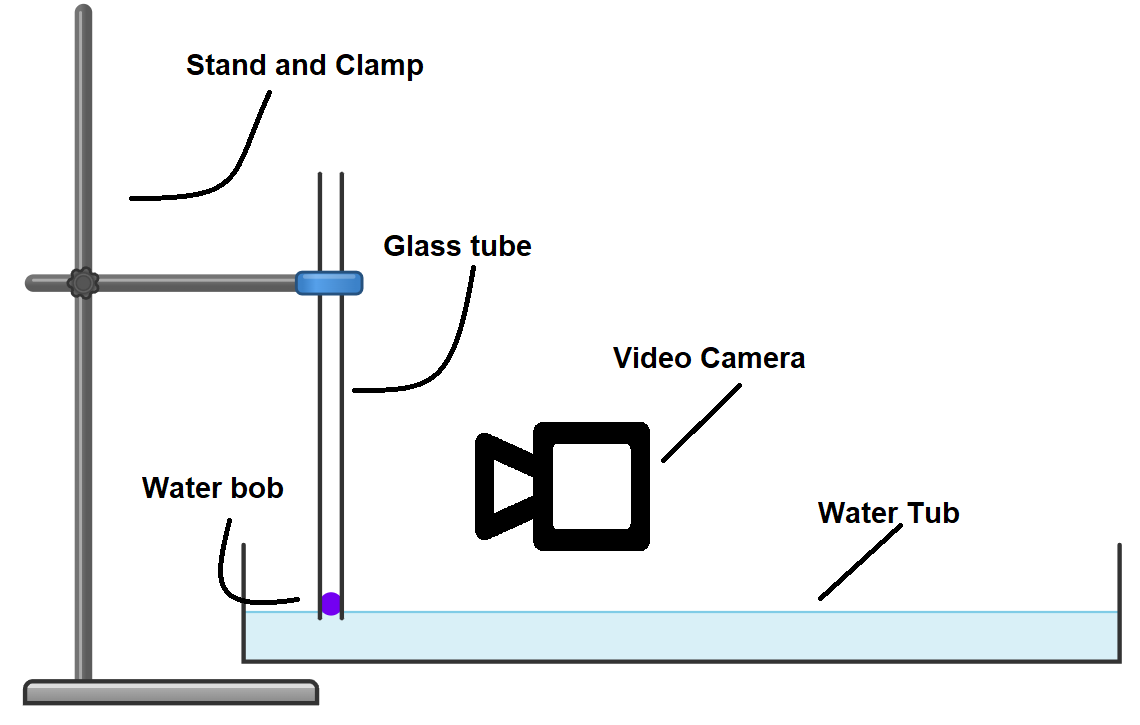
\includegraphics[width=\textwidth]{images/diagram.PNG}
      \caption{}
      \label{fig:setup}
    \end{subfigure}%
    \begin{subfigure}[b]{.5\textwidth}
      \centering
      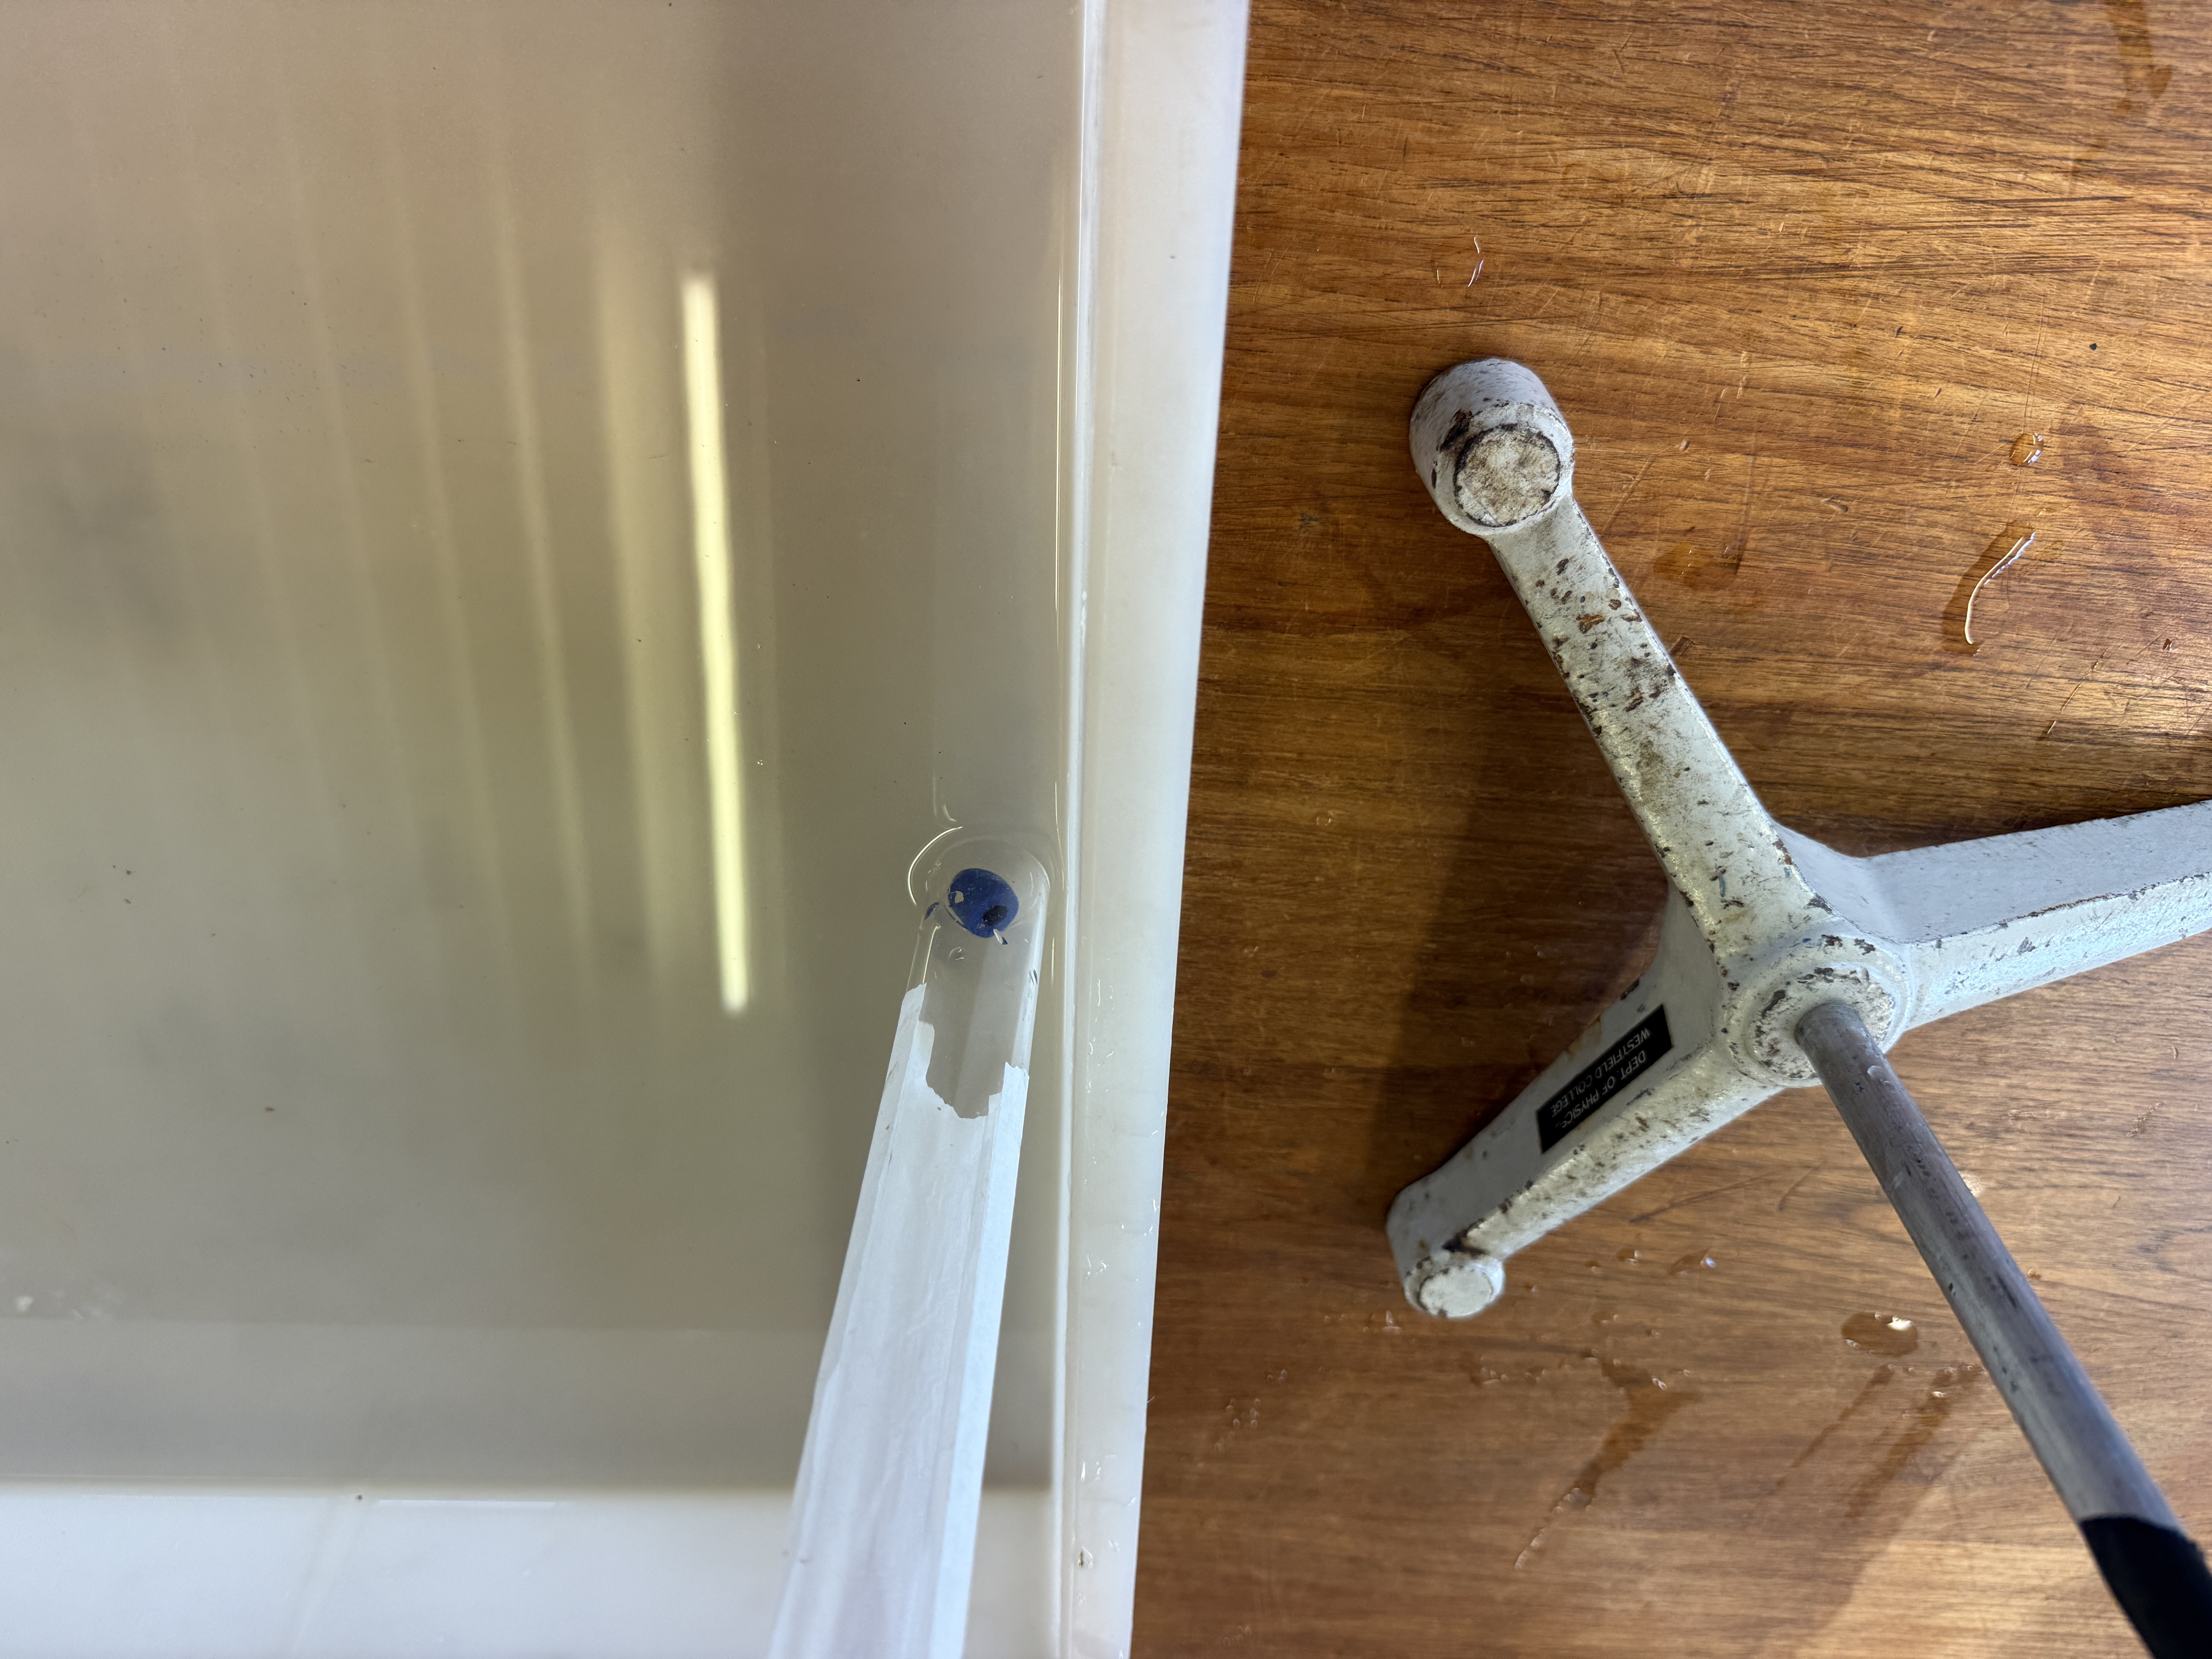
\includegraphics[width=\textwidth]{images/IMG_0244.png}
      \caption{}
      \label{fig:det-setup}
    \end{subfigure}
    \caption{(\textbf{a}) Diagram of equipment setup with detector on the left-hand side of the container. (\textbf{b}) close-up photograph of detector setup.}
    \label{fig:eqip-setup}
\end{figure}



\section{Machine Learning Model Training}
\label{sec:ML-training}

Water level sensors act as analogues for GW detectors in this experiment. Our goal with the water level sensors is to determine the TDoA between three or more detectors in order to triangulate the position of the source. Once the camera has recorded the motion of the bob it must be processed by a ML model in order to gather positional data of the bob. 

The model used is the YOLOv8 model by Ultralytics \cite{ultralytics_yolov8_nodate}, an object detection model capable of detecting objects in real time through videos and through images. The ML model is trained by manually labelling the object using the \href{https://roboflow.com/}{Roboflow} online ML training tool. This is done by simply drawing a box around the object and giving the object a name, as done in \ref{fig:train-frame}, most of the frames will be used to train the model whereas some will be used to verify the model against some test frames which aren't labelled.

Once the frames have been used to train the model, it outputs performance metrics to evaluate its accuracy in identifying objects, shown on top of the bounding box in Figure \ref{fig:det-frame}. One key metric is precision, which quantifies the model’s confidence in correctly detecting objects. This value improves as the model trains on more data, with the ideal scenario being a precision as close to 1.0 as possible. During training, the model generates a plot of precision against the number of frames processed, illustrating how the metric increases over time. Figure \ref{fig:AP} demonstrates this progression, highlighting the model’s improving detection capability.

After training, the model produces output similar to Figure \ref{fig:det-frame}, along with performance metrics that assess its accuracy. The most critical of these is the \ac{AP} value, which ``computes the area under the precision-recall curve, providing a single value that encapsulates the model's precision and recall performance" \cite{noauthor_yolo_nodate}. A higher AP value, ideally nearing 1, indicates greater confidence in object detection. This metric is visualized in Figure \ref{fig:AP}, where the trend reflects the model's strengthening performance as it processes more training data.

\begin{figure}[h!]
    \centering
    \begin{subfigure}[b]{.7\textwidth}
      \centering
      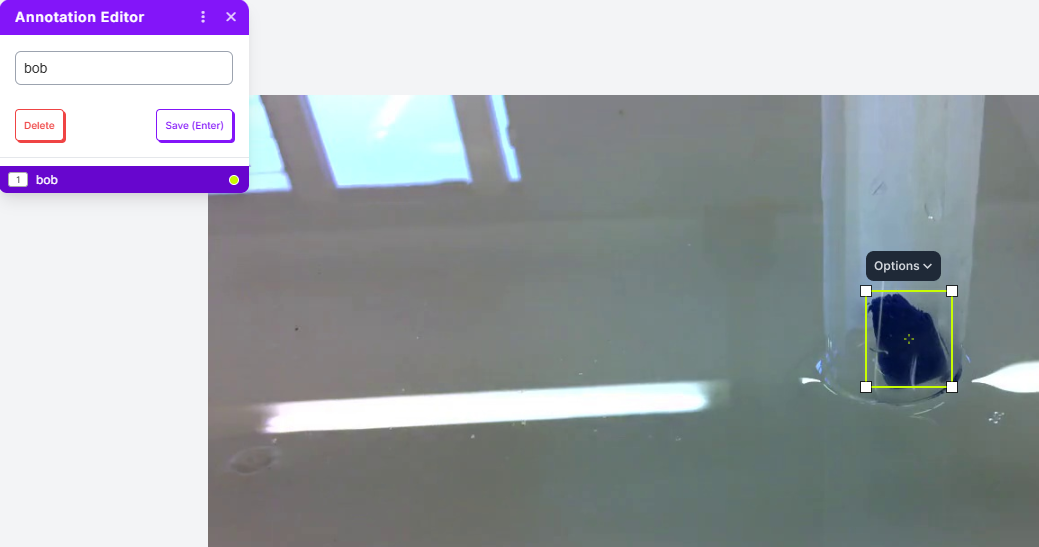
\includegraphics[width=\textwidth]{images/labelled-frame.PNG}
      \caption{}
      \label{fig:train-frame}
    \end{subfigure}%
    \begin{subfigure}[b]{.3\textwidth}
      \centering
      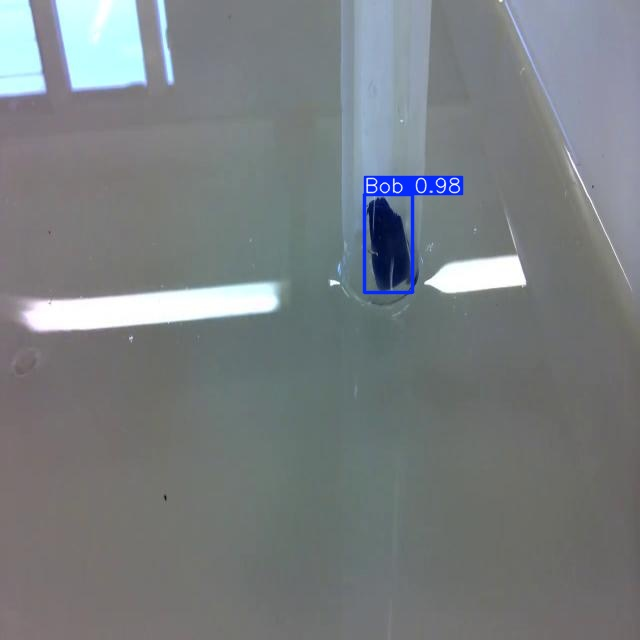
\includegraphics[width=\textwidth]{images/detected-frame.jpeg}
      \caption{}
      \label{fig:det-frame}
    \end{subfigure}
    \caption{(\textbf{a}) Process of labelling frames to train ML model on. (\textbf{b}) Frame showing the foam bob being detected through the ML model. The float value represents the accuracy of the detection from the ML model.}
    \label{fig:eqip-setup}
\end{figure}

\begin{figure}
    \centering
    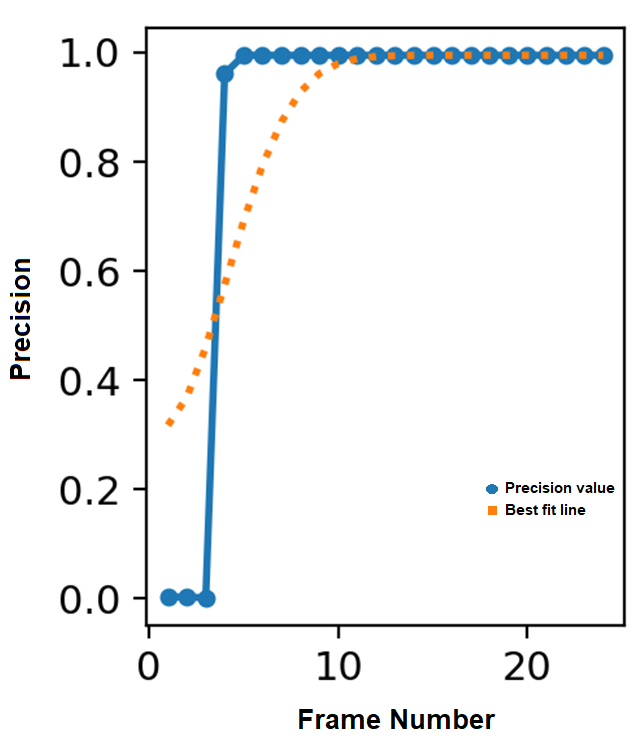
\includegraphics[width=0.5\linewidth]{images/Untitled-12.png}
    \caption{Precision value of detected object representing how "confident" the model is}
    \label{fig:AP}
\end{figure}



\section{Data Collection and Processing}
\label{sec:3.4}

\begin{figure}[h!]
    \centering
    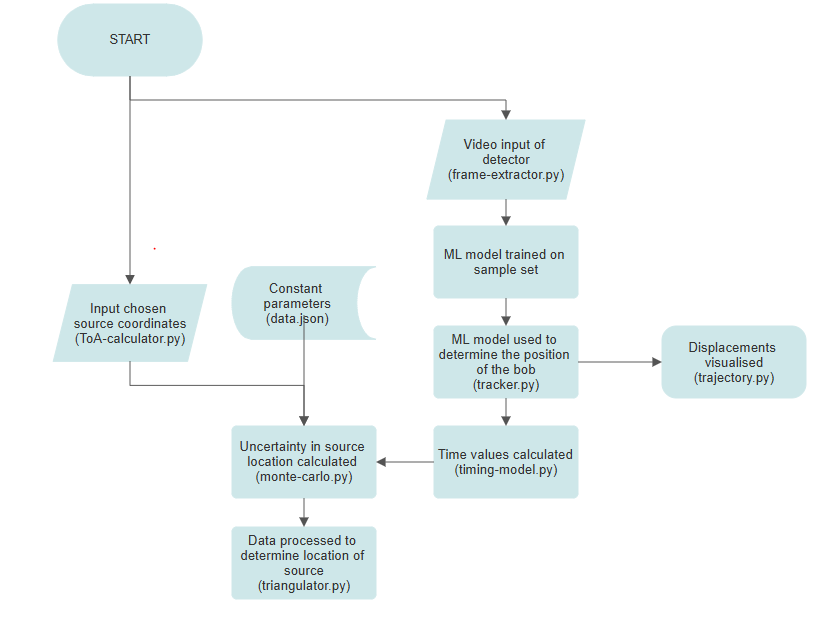
\includegraphics[width=0.9\linewidth]{images/flow.PNG}
    \caption{Flow chart of how each file is used to determine the location of the source}
    \label{fig:flow}
\end{figure}

Once the model has been trained and the precision values are close to $1.0$ it can be applied to a video recording of our GW detector analogue. The recorded video is extracted frame by frame and stored into a separate folder \cite{boxer_2025_15041819} to be processed. A python file is tasked to load the file containing the trained ML model and process each image in a sequential, marking a bounding box around the object and recording the $x,y $ coordinates of the centre of the box to be stored in an external data (JSON) file.

This JSON file contains the data necessary to determine at what time did the detector observe the GW event (through the use of frame counting as the camera records at 30 FPS) through plotting the position of the bob as it moves along in time where any significant displacements indicate a wave. 

